% =============================================================================================
% STANDALONE EXPORT OF §5 FOR EXTERNAL COLD REVIEW.
%
% Contains §5 exactly as it stands in main.tex, with its figure. Nothing is re-typed for this
% export, so it cannot drift from the manuscript: the figure float lives in sections/05_figures.tex,
% which main.tex and this file both \input.
%
% Build:  tectonic -X compile paper/review_s5.tex
% =============================================================================================
\documentclass[10pt]{article}
\usepackage{preprint}

\author{}
\date{}

\begin{document}

% §5 references three things outside this export, all in §7 and §8. Bind each label to the number
% it carries in the manuscript so every reference resolves to what a reader of the full paper
% would see.
\makeatletter
\@namedef{r@sec:lim-universe}{{7.5}{1}{One exchange, one venue, one year of scored data}{subsection.7.5}{}}
\@namedef{r@sec:lim-universe@cref}{{[subsection][5][7]7.5}{1}}
\@namedef{r@sec:lim-features}{{7.7}{1}{The microstructure leg is narrower than ``microstructure'' suggests}{subsection.7.7}{}}
\@namedef{r@sec:lim-features@cref}{{[subsection][7][7]7.7}{1}}
\@namedef{r@sec:repro}{{8}{1}{Reproducibility and verification}{section.8}{}}
\@namedef{r@sec:repro@cref}{{[section][8][]8}{1}}
\makeatother

\setcounter{section}{4}   % so §5 numbers as §5, matching the manuscript
\setcounter{figure}{6}    % Figures 1--6 precede this section
\setcounter{table}{0}

{\centering
{\normalsize\textsc{Section 5 --- export for external review}}\\[0.5em]
{\Large\bfseries Capacity Eviction in Reconstruction-Trained Tokenizers}\\[0.4em]
{\small\color{tolgrey} Draft of \today\ --- section text frozen pending review}\\[1.6em]
}

\noindent\textbf{Note to the reviewer.} This is \S5 of a paper in preparation, exported verbatim
from the manuscript with its figure. Numbering matches: \S5.1--\S5.7 and Figure~7. References to
\S7 and \S8 point outside this export and are bound to their manuscript numbers. \S5 is being
reviewed alongside \S7, which carries the limitations these facts imply; where \S5 states a scope
boundary it names the \S7 subsection that owns it rather than arguing it here.

\medskip
\noindent\textbf{Every number in this section was re-verified against its artifact by script}
before export --- 25 of 25, re-read from the milestone record, the lake-surface receipt, the
design-inputs receipt and the pinned constants imported live, rather than transcribed from an
earlier draft.

\medskip
\noindent\textbf{What we would most like challenged.} (i) Whether \S5.1's construction actually
removes survivorship bias, or only the most visible part of it --- the universe is bootstrapped
from the dump index rather than a live instrument list, but an instrument still had to list on
this venue to be in it. (ii) Whether \S5.2's disclosure is placed strongly enough: the feature
vector is 16 wide and 13 live, and three specified dimensions are constant-zero on every bar.
(iii) Whether the causal-normalization argument in \S5.3 is complete, or whether there is a
lookahead path the planted-leak tests do not cover. (iv) Whether \S5.4's $99.0\%$ microstructure
availability is really enough to say the placebo comparison is not confounded by absence.
(v) Whether the $41$-versus-$17$ delisting distinction in \S5.5 is stated clearly enough to
survive being quoted out of context. (vi) Any number that does not follow from what is stated.

\bigskip
\hrule
\bigskip

% =============================================================================================
% §5 Data.  Every number carries its artifact.
%
% The section's job is not to describe a dataset but to let a referee decide whether the dataset
% can support the claim -- so the ordering runs: what the universe is and why it is not
% survivorship-filtered, what a bar contains and what it does NOT, how normalization stays causal,
% what the quality gates cost, and what the experiment actually reads out of all of it.
% =============================================================================================
\section{Data}
\label{sec:data}

\subsection{One venue, and the universe chosen from inside it}
\label{sec:data-universe}

Every instrument is a USDT-margined perpetual future on Binance, sampled at one-minute frequency
over the four years \mbox{2021-01-01} to \mbox{2025-01-01}. Two public sources are combined per
bar: the klines dump supplies open, high, low, close, volume and quote volume; the aggregated-trades
dump supplies the signed trade statistics that the microstructure block is built from. No paid feed
and no order book is involved, which is a scope limit (\cref{sec:lim-features}) and also the reason
the corpus is reproducible by anyone.

The symbol set is bootstrapped \emph{from the data} rather than from the exchange's live instrument
list, and that choice is the one that decides whether the universe is survivorship-biased. A live
instrument listing contains only instruments that still exist; selecting from it silently deletes
every instrument that failed, which is the single most common way a backtest flatters itself. We
instead scan the S3 index of the aggregated-trades dumps once, which yields per symbol, without
downloading a single bar, the set of monthly dumps that exist. From that: the listing month is the
first dump, and an instrument is treated as delisted when its last dump trails the newest global
month. Ranking by total aggregated-trades bytes --- a liquidity proxy available from the same
index --- and taking the top 200 gives the universe: \textbf{200 symbols, of which 41 were already
delisted at the time of the scan}, each contributing only its $[\text{listing}, \text{delisting})$
bars.
% artifact: docs/milestone4b_universe_ingest.md §2 — dump-index bootstrap; "200 symbols selected, 41 delisted"; config/universe_full.yaml carries listing/delisting per symbol with a recorded config_hash

One detail in that rule is worth stating because it changes three symbols. A dump index is published
with lag, so an instrument that is merely a month behind the freshest global dump is not delisted ---
it is late. The delisting test therefore carries a one-month publish-lag tolerance, which corrected
three symbols relative to a zero-tolerance comparison. Without it the universe would have carried
three phantom delistings.
% artifact: docs/milestone4b_universe_ingest.md §2 and §7 — publish-lag tolerance, "corrected 3 symbols vs a zero-tolerance comparison"

The realized ingest is \textbf{304{,}625{,}181} bars across all 200 symbols. That is below the
$500$M--$1$B band the blueprint nominated, and we flag it rather than quietly re-describe the band:
200 instruments over the fullest available window, many of them partial-coverage through late
listing or delisting, lands near 300M. We regard it as adequate rather than merely acceptable, for
a reason that is about the model and not about the data --- a 21M-parameter backbone saturates
well below this, so the lake is bought for regime and cross-sectional breadth rather than as
training fuel. Reaching the nominal band would need roughly 320 instruments at proportional
bandwidth, and would not train a better model.
% artifact: runs_manifest/m6_c15b_lake_surface_check.json :: sampling.{bars = 304625181, symbols = 200, fraction_of_lake = 1.0, shards_sampled = ALL}
% artifact: docs/milestone4b_universe_ingest.md §4 exit-gate row — band flagged, corpus-purpose recorded in manifest metadata

\subsection{What a bar is, and what three of its dimensions are not}
\label{sec:data-features}

Each bar is reduced to a $16$-dimension feature vector. Seven dimensions are price shape and
liquidity: log close-to-close return, log range, body fraction, upper and lower wick fractions, log
volume and log quote volume. Six are the microstructure block, computed from aggregated trades:
trade-flow imbalance $(v_{\text{buy}} - v_{\text{sell}})/(v_{\text{buy}} + v_{\text{sell}})$,
signed count imbalance, log trade count, log mean trade size, trade-size dispersion, and large-trade
share. These six --- indices $7$ through $12$ --- are the block the ablation varies, and the first
of them is the quantity the paper is about.
% artifact: src/trikaal/constants.py :: FEATURE_NAMES (16 entries), MICRO_DIMS_IDX
% artifact: src/trikaal/data/features.py :: raw_feat[:, 7] = (v_buy - v_sell) / (v_agg + EPS_CNT), and rows 0--12 above it

The remaining three dimensions --- funding rate, log open interest and its change, indices $13$ to
$15$ --- are specified, wired through every transform, and \textbf{structurally absent}. The v1
ingest covers klines and aggregated trades only, so on all $304{,}625{,}181$ bars those three
columns have standard deviation exactly $0.0$ and their masks are set on $100\%$ of rows. We state
this here rather than in a footnote because the natural reading of ``a 16-dimensional
microstructure vector for perpetual futures'' is that funding and open interest are in it, and
they are not. The vector is $16$ wide and $13$ live. \Cref{sec:lim-features} carries what that
costs.
% artifact: docs/m6_prereg.md §7 v1.6.16 — x_13/14/15 stddev exactly 0.0, m_13/14/15 masked on 100% of bars
% artifact: src/trikaal/constants.py :: MASK_BITS_PERP = (13, 14, 15)

Every feature carries a companion mask bit, and the mask travels with the value through every
downstream transform. That pairing is not bookkeeping: a defect found in review had the placebo
shuffle permuting values while leaving masks in place, which would have stranded fill values on
valid bars and real values on masked ones. It was fixed before any training run.
% artifact: docs/BUILD_RECORD.md §2, D6 — "the placebo shuffle broke (value, mask) pairing"

\subsection{Normalization that cannot see forward}
\label{sec:data-causal}

Feature scales in this market move by orders of magnitude across four years, so the unbounded
dimensions are normalized rather than used raw. The normalization is where lookahead usually
enters a financial pipeline, through a statistic fitted on the whole sample and then applied to its
own training region, so the rule here is absolute: every statistic used for bar $t$ is computed
from data available at the close of bar $t$.

Nine dimensions --- the unbounded, scale-varying ones --- receive a causal exponentially weighted
z-score, at a half-life of $1{,}440$ bars (one day) for the fast group and $5{,}760$ bars (four
days) for the slow volume and open-interest group. Seven dimensions are already bounded or
relative, and are clipped only. Everything is clipped last to $[-5, +5]$ as an outlier guard. The
volatility scale $\sigma_t$ that the prediction targets are expressed in is built causally from
raw returns within a segment, on the same rule.
% artifact: src/trikaal/constants.py :: Z_SCORED_IDX (9 entries), BOUNDED_IDX (7), CLIP_LO/CLIP_HI = -5.0/+5.0, FAST_ZSCORE_IDX, SLOW_ZSCORE_IDX
% artifact: src/trikaal/data/config.py :: half_life_fast = 1440, half_life_slow = 5760; effective_n_warm(H) = max(n_warm, H//8); effective_n_warm_vol() = max(n_warm_vol, half_life_fast)

Each statistic needs a warm-up before it is trustworthy, and warmed-up bars are dropped rather than
back-filled. The cost is small and it is measured, not estimated: on the three thinnest instruments
in the universe the warm-up drop is $809$ of $279{,}930$ bars, $811$ and $809$ respectively ---
about $0.3\%$ --- because most instruments are long single segments and the warm-up is a one-time
tax at the start of each.
% artifact: docs/milestone4b_universe_ingest.md §4.1 spot-check — ZROUSDT 809/279,930 (0.3%), TURBOUSDT 811, NOTUSDT 809
% NOTE: that §4.1 prose calls this "the ~800-bar z-score warm-up", but the pinned constants give a
% 180-bar fast z warm-up, 720-bar slow, and 1,440-bar volatility warm-up (effective_n_warm_vol =
% max(30, 1440)), confirmed at runs_manifest/m6_c15b_lake_surface_check.json ::
% question_2....effective_n_warm_vol = 1440. The MEASURED drop of ~809 bars is what we quote; the
% "~800-bar warm-up" description is not reconciled with the constants and is not repeated here.

Causal safety is not asserted, it is a required continuous-integration gate. The test suite plants
lookahead leaks of several kinds --- a global one, a localized divisor leak, and a survivorship
leak in the target-validity flag --- and asserts that the exhaustive sweep catches each. One of
those tests exists specifically to show that a \emph{sampling} check misses the localized leak that
the exhaustive check catches, so the gate cannot be quietly weakened to a sampler. During ingest
the same sweep ran in-line on real cross-sections and a red result raised a fatal error before
anything was recorded.
% artifact: tests/data/test_causal_safety.py :: test_global_planted_leak_is_caught, test_localized_divisor_leak_caught_by_exhaustive_but_missed_by_sampler, test_localized_survivorship_leak_in_target_valid_is_caught, test_mask_is_strictly_causal
% artifact: docs/milestone4b_universe_ingest.md §6 — in-line sweep GREEN at scale on [live] HOOKUSDT, [tail] YFIIUSDT, [live] AXSUSDT; 100% coverage, 6,398 checks each; red raises FatalIngestError

\subsection{What the quality gates cost}
\label{sec:data-quality}

Of the $304{,}625{,}181$ bars, \textbf{$303{,}283{,}972$ ($99.56\%$) are usable by the OHLCV-only
arm} after warm-up and quality masking, and \textbf{$300{,}311{,}536$ ($98.58\%$) are usable by the
microstructure arms}. The ratio between those --- microstructure availability given price
availability --- is $99.0\%$ universe-wide, and no instrument falls below $0.7$. Across the
universe, $0.175\%$ of bars are stale and $0.376\%$ have zero volume.
% artifact: docs/milestone4b_universe_ingest.md §4.1 DQ table — total 304,625,181; OHLCV-usable 303,283,972 (99.56%); +micro-usable 300,311,536 (98.58%); micro-availability 99.0%, 0 symbols below 0.7; is_stale 0.175%, zero-vol 0.376%
% artifact: runs_manifest/m6_c10_micro_density.json :: symbols_with_zero_unmasked_per_dim = {} for dims 7--12; per_dim_total_unmasked ~ 3.0e8 each

That second number is the one that matters for the placebo. If microstructure were missing on a
large fraction of bars, cell 4 and cell 5 would differ in coverage as well as in content, and the
comparison the paper rests on would be confounded by absence rather than by information. At
$99.0\%$ availability with no starved instrument, it is not.

Forty-three instruments are thin, by a joint rule --- fewer than half the median usable bars, or
more than $10\%$ stale. Inspecting them rather than dropping them: almost all are recent 2024
listings with $280$k--$500$k bars and microstructure availability near $1.00$, so they are thin by
\emph{age}, not by quality. The single genuinely illiquid instrument is a delisted one at $2.5\%$
stale and $2.6\%$ zero-volume. All 43 remain in the lake; thinness is handled as a sampling weight
in the training draw, not as a deletion.
% artifact: docs/milestone4b_universe_ingest.md §4.1 — 43 thin-coin candidates, rule and per-symbol table at docs/_m4b_dq_table.md; FRONTUSDT stale 2.5% / zero-vol 2.6%

\subsection{Coverage, and the survivorship we did not remove}
\label{sec:data-coverage}

\Cref{fig:coverage} is the whole universe as a symbol-by-month raster: $7{,}024$ of a possible
$9{,}600$ symbol-months are present. The left staircase is instruments listing at different dates.
The right edge is ragged because instruments that stop trading are \emph{kept} in the lake, and
their absence afterwards is real absence rather than a filter. A survivorship-cleaned universe
renders as a solid rectangle, which is precisely the artefact the panel exists to demonstrate we
did not create. Two instruments have interior gaps rather than truncated tails and appear as
internal white streaks.

Two delisting counts appear in this project and they count different things, so we state both. The
ingest record's \textbf{41} is the number of instruments known to be delisted as of the index scan,
at any date. The \textbf{17} in \cref{fig:coverage} is the number whose data ends \emph{inside} the
four-year window, which is all a raster over that window can show; the remaining $24$ delist after
2024-12 and are complete here. The figure and this section therefore say ``stop trading inside the
window'' and never ``delisted''.
% artifact: paper/figures/make_fig7_coverage.py header — the 2026-08-09 reconciliation, spot-checked against the ingest note's own worked examples (AGIXUSDT, AUDIOUSDT); the note quotes the first ABSENT month, the lake stores the last PRESENT one
% artifact: coverage raster enumerated from processed/universe_bars/symbol=*/month=* at render time, 200 x 48

Survivorship is owned, not solved. Retaining failed instruments removes one bias; it does not
remove listing bias, since an instrument must have been listed on this venue at all to enter the
universe. \Cref{sec:lim-universe} carries that.

\subsection{Storage, provenance, and what makes a past prediction reconstructible}
\label{sec:data-provenance}

The reduced lake is Hive-partitioned Parquet under \texttt{(symbol, frequency, month)}, queried
through DuckDB. It was first written per-day, at $211{,}595$ files, which made per-symbol globbing
pathological; compaction to one file per symbol-month gives $7{,}024$ files and $15$\,GB. The
compaction was proven content-preserving rather than assumed: all $200$ per-symbol dataset hashes
were re-derived from the compacted lake and the universe Merkle root recomputed, with zero
mismatches and an unchanged root. Identical features, masks and timestamps imply an identical
causal result, so the hash comparison subsumes a re-run of the causal sweep.
% artifact: docs/milestone4b_universe_ingest.md §4.1 lake-compaction entry — 211,595 -> 7,024 files, 23 GB -> 15 GB, 0 hash mismatches, Merkle unchanged; scripts/compact_lake.py

Every dataset is content-hashed and the universe carries a single Merkle root over the lake,
\texttt{sha256:5dfd667d05b97bda\ldots}, recorded in the manifest alongside per-symbol listing and
delisting dates and a corpus-purpose note.
% artifact: docs/milestone4b_universe_ingest.md §4 — Universe Merkle sha256:5dfd667d05b97bda... (200-symbol; the 199-symbol first-pass intermediate was 9400a271...)

Raw dumps are not retained, and that is a deliberate position rather than a shortcut. The Merkle
root and the per-symbol hashes are taken over the \emph{reduced} lake, which is the artifact we
keep; the Binance SHA-256 of every raw shard is recorded for provenance only. Re-pulling raw and
re-running a deterministic reducer reproduces the recorded lake hash --- the reducer was proven
byte-identical at the preceding milestone --- so reproducibility survives eviction of $503$\,GB of
raw input.
\Cref{sec:repro} states exactly which parts of the pipeline are bit-exact and which are not.
% artifact: docs/milestone4b_universe_ingest.md §4.1 "Reproducibility survives raw eviction"; peak raw cache 30 GB, 503 GB cycled through eviction to raw 0

\subsection{What the experiment reads}
\label{sec:data-slice}

The lake is broader than the experiment. Of the $200$ instruments, the headline metric is scored on
$40$; the four-year window is split at its $0.7$ point, on 2023-10-20, into a training region and a
forward region, and the forward region is cut into six blocks of which block $0$ is spent selecting
the execution filter and excluded. The headline is therefore computed on blocks $1$ through $5$ ---
roughly 2024-01-01 to 2025-01-01, one year, $35{,}063$ stride-$15$ periods per instrument --- on a
region no selection step has seen. The other $160$ instruments and the preceding three years are
lake breadth and training data, not evaluation breadth, and \cref{sec:lim-universe} states what
that leaves unestablished.
% artifact: runs_manifest/m6_mde_inputs.json :: symbols_sampled (40 entries), primary_region_ms = [1704132000000, 1735689600000], n_blocks = 6, h15_pooled.T = 35063; conformance hard-asserts (val_block = 0, n_blocks = 6)

% The figure belonging to §5. Held in its own file so main.tex and review_s5.tex share one
% copy and the export cannot drift from the manuscript.
\begin{figure}[t]
  \centering
  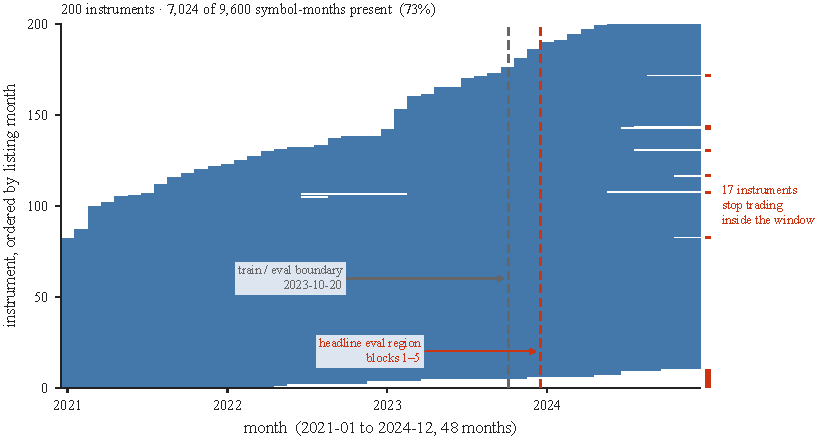
\includegraphics[width=\textwidth]{figures/fig7_coverage.pdf}
  \caption{\textbf{Survivorship is owned, not filtered away.} Month-by-month presence for all $200$
  instruments over the four-year window, ordered by listing month: $7{,}024$ of a possible
  $9{,}600$ symbol-months are present. The left staircase is instruments listing at different
  times; the right edge is ragged because instruments that stop trading are \emph{kept}, and $17$
  of them stop inside this window. A survivorship-filtered universe would render as a solid
  rectangle, which is the artefact this panel exists to show we did not create. Two instruments
  have interior gaps rather than truncated tails and appear as internal white streaks. The two
  dashed rules are the committed fold plan: training ends at the first, and the headline metric is
  scored only to the right of the second. Note that $17$ counts instruments whose data ends inside
  the window; the ingest record's $41$ counts every instrument known to be delisted at any date,
  including $24$ that delist after this window closes.}
  \label{fig:coverage}
\end{figure}


\clearpage
\bibliographystyle{plainnat}
\bibliography{refs}

\end{document}
